\section{Theorie}
\label{sec:Theorie}
Ein Fadenpendel der Länge $l$ schwinge im Gravitationspotential der Erde. \\ 

\noindent Mit $\vec{r} = \left(\begin{array}{c} l \cos(\phi) \\ l \sin(\phi) \end{array} \right)$ und $\dot{\vec{r}} =\left(\begin{array}{c} -l \sin(\phi) \\ l \cos(\phi) \end{array} \right)$ \\

\noindent folgt aus der kinetischen Energie $T = \dfrac{m}{2} v^2 = \dfrac{m}{2} \dot{r}^2$, \\
der potentiellen Energie $V = mgy = mg\sin(\phi)$ und der Lagrange-Funktion $\mathscr{L} = T - V$ mit den Euler-Lagrange-Gleichungen die Bewegungsgleichung \\

\noindent $\ddot{\phi} = \dfrac{g}{l}\sin{\phi}$. \\

Die Kleinwinkelnäherung $\sin{\phi}=\phi$, kleine Winkel bezeichnen im Normalfall Winkel mit $\phi \leq 10°$ \cite{wiki:xxx}, liefert die DGL $\ddot{\phi} = \dfrac{g}{l}\phi$ mit der Lösung \\ 
$\phi(t) = C_1 \cos(\omega_0t) + C_2 \sin(\omega_0t)$ , $\omega_0=\sqrt{\dfrac{g}{l}}$. \\

Werden zwei Fadenpendel mit einer Feder aneinander gekoppelt, schwingen sie nicht länger unabhängig voneinander, es stellt sich ein zusätzliches Drehmoment ein. \\

\noindent Dabei ist $M_1=D_F(\phi_2-\phi_1)$ und $M_2=D_F(\phi_1-\phi_2)$. \\

Unter diesen Drehmomenten ergibt sich mit dem Trägheitsmoment $J=mL^2$ der Pendel ein System gekoppelter Differentialgleichungen. Es gilt\\

\noindent $J\ddot{\phi_1} + D\phi_1 = M_1$ \\

\noindent $J\ddot{\phi_2} + D\phi_2 = M_2$. \\

So stellen sich je nach Anfangsbedingung unterschiedliche Schwingmoden ein. Dabei unterscheidet man gleichsinnige, gegensinnige und gekoppelte Schwingungen. \\

\newpage

Für \textbf{gleichphasige Schwingungen}, sprich $\phi_1=\phi_2$, stellt sich für zwei identische Pendel die bereits aus der Schwingung einzelner Pendel bekannte Frequenz \\ 
$\omega_+=\sqrt{\dfrac{g}{l}}$ mit der Periodendauer 
\begin{equation}
T_+ = 2\pi \omega_+ = 2\pi \sqrt{\dfrac{l}{g}} \text{\, ein.}
\label{eq:T_+}
\end{equation}

\begin{figure}
    \centering
    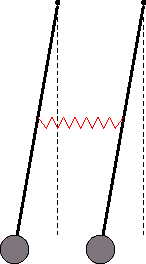
\includegraphics{v106_abb1.pdf}
    \caption{Gleichphasige Schwingung}
\end{figure}

Bei entgegengesetzten Anfangsauslenkungen ($\phi_1=-\phi_2$) spricht man von einer \\ 
\textbf{gegenphasige Schwingung}. Die Schwingfrequenz $\omega_-$ ergibt sich dann zu \\
$\omega_- = \sqrt{\dfrac{g+2K}{l}}$, wobei $K$ die Kopplungskonstante der Feder darstellt.
Die Periodendauer ist dann 
\begin{equation}
    T_- = 2 \pi \omega_- = 2 \pi \sqrt{\dfrac{l}{g+2K}}\text{.}
\label{eq:T_-}
\end{equation}

\begin{figure}
    \centering
    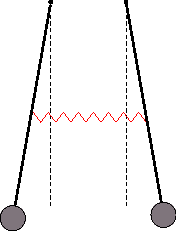
\includegraphics{v106_abb2.pdf}
    \caption{Gegenphasige Schwingung}
\end{figure}

\textbf{Gekoppelte Schwingungen} bezeichnen Schwingungen, bei denen für eine der Anfangsauslenkungen $\phi_n = 0$ gilt. Eines der Pendel befindet sich also zu Beginn in Ruhe.
Das schwingende Pendel beginnt, seine Energie auf das ruhende Pendel zu übertragen, seine Amplitude nimmt also langsam ab, während die des zunächst ruhenden Pendels immer weiter zunimmt und ihr Maximum erreicht, sobald das andere Pendel ruht.
Dieser Vorgang der Energieübertragung wiederholt sich immer wieder, die Zeit zwischen zwei Ruhezeiten eines Pendels wird dabei als Schwebungsdauer $T_S$ mit der Schwebungsfrequenz $\omega_S$ bezeichnet. \\
Dabei gilt $\omega_S= \omega_+ -\omega_-$ und
\begin{equation}
    T_S = \dfrac{T_+ T_-}{T_+ - T_-} \text{.}
\label{eq:T_S}
\end{equation}

\begin{figure}
    \centering
    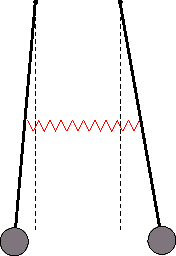
\includegraphics{v106_abb3.pdf}
    \caption{Gekoppelte Schwingung}
\end{figure}

Der Kopplungsgrad $K$ der beiden Pendel ist dabei definiert als
\begin{equation} 
    K := \dfrac{\omega_-^2-\omega_+^2}{\omega_-^2 + \omega_+^2} = \dfrac{T_+^2 - T_-^2}{T_+^2 + T_-^2} \text{.}
\label{eq:Kopplungsgrad}
\end{equation} \cite{ap01}



